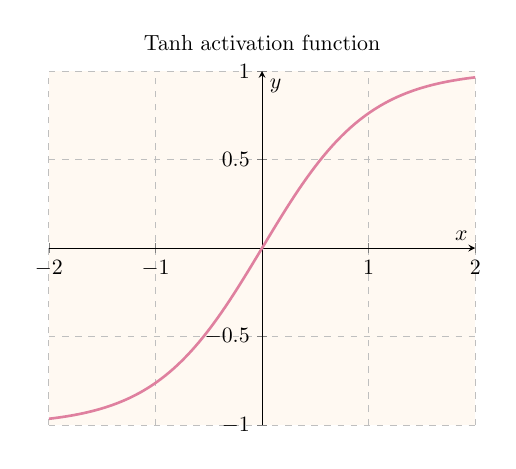
\begin{tikzpicture}[scale=0.79]
\begin{axis}[
    clip = false,
    axis lines = middle,
    xlabel = $x$,
    ylabel = $y$,
    xtick = {-2, -1, 1, 2},
    ytick = {-1, -0.5, 0.5, 1},
    ymajorgrids = true,
    xmajorgrids = true,
    grid style = dashed,
    xmin=-2, xmax=2,
    ymin=-1, ymax=1,
    title = {Tanh activation function},
    axis background/.style={fill=orange!5}
]
%Below the purple parabola is defined
\addplot [
    domain=-2:2, 
    samples=100, 
    color=purple!50,
    very thick,
]
{(e^x - e^(-x))/(e^x + e^(-x))};

\end{axis}
\end{tikzpicture}